\documentclass[UTF8, a4paper]{ctexart}
\usepackage[margin=1in]{geometry} % 页边距调整
\usepackage{ctex}
\usepackage{array, amsmath, amssymb}

\usepackage{booktabs, tabularx, multirow, multicol} % 表格拓展支持
\usepackage{graphicx, subfigure, float} % 图片排版支持

\usepackage{algorithm, algpseudocode} % 伪代码支持
\renewcommand{\algorithmicrequire}{\textbf{Input:}}  
\renewcommand{\algorithmicensure}{\textbf{Output:}} 

\usepackage{tikz, mathpazo} % 基本绘图支持
\usepackage{flowchart} % 流程图支持
\usepackage{pgf-umlcd} % UML类图支持
\usetikzlibrary{arrows, shapes, chains, shapes.geometric}

\usepackage{listings} % 代码块支持
\usepackage{xcolor}
\lstset{
	language		= c++,
	backgroundcolor	= \color{white},
	basicstyle		= \footnotesize\ttfamily,
	keywordstyle	= \color{blue},
	stringstyle		= \color{red!58!blue!82}\ttfamily,
	commentstyle	= \color{darkgray},
	rulesepcolor	= \color{red!20!green!20!blue!20},
	columns			= fullflexible,
	breaklines		= true,
	captionpos		= b,
	tabsize			= 4,
	frame			= single,
	escapeinside	= {\%*}{*)}
}
%%示例
% \begin{lstlisting}[caption={}]
% #include <iostream>
% int main(int argc, char *argv[]) {
% 	std::cout << "Hello World!" << std::endl;
% 	return 0;
% }
% \end{lstlisting}

\usepackage{datetime} %日期
\renewcommand{\today}{\number\year{年}\number\month{月}\number\day{日}}

\begin{document}

\begin{center}
	\zihao{3}《数据结构》实验报告
\end{center}
\zihao{5}

\newcolumntype{Y}{>{\raggedleft\arraybackslash}X}
\noindent\begin{tabularx}{\textwidth}{XcY}
	  {班 级:}\;\underline{DL062123}
	& {姓 名:}\;\underline{项乔栋}
	& {学 号:}\;\underline{2021302468} \\
	  {邮 箱:}\;\underline{13282135976@sina.cn}
	& {日 期:}\;\underline{\today}
	& {编 号:}\;\underline{DS11}
\end{tabularx}
~\\

\noindent\textbf{$\circledcirc$
实验题目:\quad{最短路径}} \par
\noindent\textbf{$\circledcirc$
实验目的:\quad{解决图论问题}} \par
\noindent\textbf{$\circledcirc$
实验内容:\quad{Floyed算法实现任意最短路径的求解}} \par

\subsection*{一、需求分析}
\noindent\fbox{
\begin{tabularx}{\textwidth}{lY}
\bf{Description}
& \parbox[t]{\linewidth}{
	用弗洛伊德算法求任意两点间的最短路径,并输出指定的m对结点间的最短路径。
} \\

\bf{Input}
& \parbox[t]{\linewidth}{
	先输入一个小于100的正整数n,然后输入图的邻接矩阵(10000表示无穷大,即两点之间没有边),最后输入两个0到n-1的整数表示两个点。
} \\

\bf{Output}
& \parbox[t]{\linewidth}{
	用弗洛伊德算法求任意两点间的最短路径,并输出这些两个点之间的最短路径。
} \\

\bf{Sample Input}
& \fbox{\parbox[t]{\linewidth}{\bf{
	\mbox{4} \\
	\mbox{0 2 10 10000} \\
	\mbox{2 0 7 3} \\
	\mbox{10 7 0 6} \\
	\mbox{10000 3 6 0} \\
	\mbox{2} \\
	\mbox{0 2} \\
	\mbox{3 0}
}}} \\

\bf{Sample Output}
& \fbox{\parbox[t]{\linewidth}{\bf{
	\mbox{0} \\
	\mbox{1} \\
	\mbox{2} \\
	\mbox{3} \\
	\mbox{1} \\
	\mbox{0}
}}}
\end{tabularx}}

\subsection*{二、概要设计}
% 摘要
\par
1.\;基本操作: \par
	CreateFromIO() $\rightarrow$ Graph \par
	\qquad\textbf{操作结果:}\;从IO流创建无向图 \par
	Floyd(G:Graph) $\rightarrow$ Array<Integer>[2] \par
	\qquad\textbf{操作结果:}\;Floyd求解所有最短路径 \par
2.\;程序模块: \par
1) 主程序 \par
2) IO支持 \par
3) Floyd 最短路径问题求解 \par
\begin{figure}[H]
	\begin{minipage}[t]{\linewidth}
		\centering
		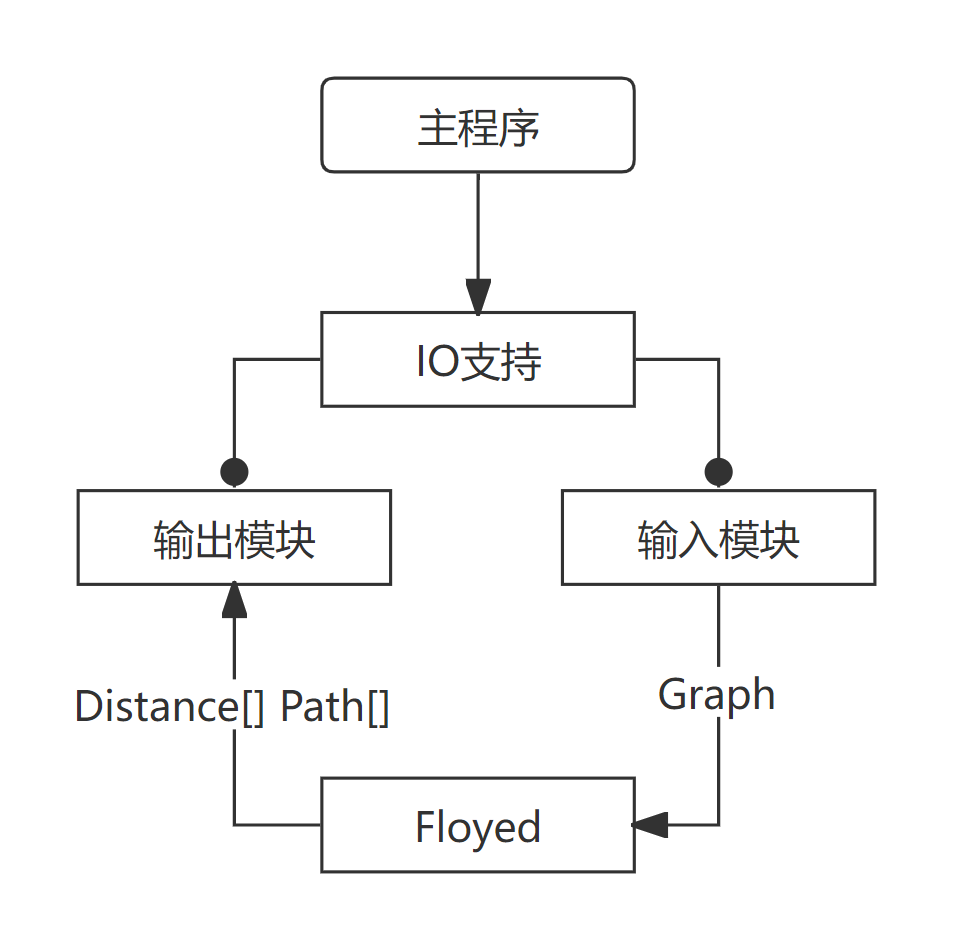
\includegraphics[width=80mm,height=85mm]{./assets/DS11-1}
	\end{minipage}
\end{figure}

\subsection*{三、详细设计}
\begin{algorithm}[H]
\begin{algorithmic}[1]
\caption{Floyd Algorithm}
\Require DG: $\mathbf{G}$
\Ensure Array<Integer>: $\mathbf{distance}$, $\mathbf{path}$
\For {$0\leq{i}<|V(\mathbf{G})|, 0\leq{j}<|V(\mathbf{G})|$}
	\State $\mathbf{distance}$[i][j] = $\mathbf{G}$[i][j]
	\State $\mathbf{path}$[i][j] = j
\EndFor
\For {k = 0 to $|V(\mathbf{G})|$}
	\For {$0\leq{i}<|V(\mathbf{G})|, 0\leq{j}<|V(\mathbf{G})|$}
		\If {i $\neq$ j and $\mathbf{distance}$[i][j] > $\mathbf{distance}$[i][k] + $\mathbf{distance}$[k][j]}
			\State $\mathbf{distance}$[i][j] = $\mathbf{distance}$[i][k] + $\mathbf{distance}$[k][j]
			\State $\mathbf{path}$[i][j] = $\mathbf{path}$[i][k]
		\EndIf
	\EndFor
\EndFor
\State return $\mathbf{distance}$, $\mathbf{path}$
\end{algorithmic}
\end{algorithm}

\subsection*{四、使用说明、测试分析与结果}
\subsubsection*{1、使用说明}
1) 本程序可以通过任意支持C++11及以上标准的编译器生成目标文件并在当前平台运行。 \par
2) 进入程序后务必依照需求的输入样式输入数据,手动输入与流式输入都是被允许的。 \par
\subsubsection*{2、测试结果与分析}
2.1\;\textbf{实际环境} \par
对于所有输入,皆为正赋权有向图,且满足输入要求中提及的条件。 \par
2.2\;\textbf{边界情况} \par
无 \par
2.3\;\textbf{测试结果} \par
目标代码通过全部测试,无需纠正 \par
\subsubsection*{3、调试过程问题分析与解决办法}
编码与测试环节皆未产生必须被处理的问题,跳过调试环节 \par
\subsubsection*{4、设计与实现的回顾讨论与分析}
简单地应用Floyd算法来解决问题,算法本身将给出最短路径长度,中继节点将给出路径信息。所有信息具备,且算法本身高度简洁,故而实现起来整体也是简单难出错。 \par
\subsubsection*{5、运行界面}
\begin{figure}[H]
	\begin{minipage}[t]{\linewidth}
		\centering
		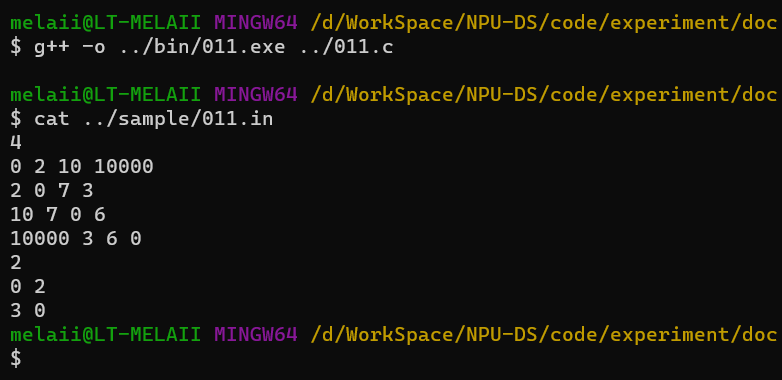
\includegraphics[width=125mm,height=60mm]{./assets/DS11-2}
		\caption{前置环境}
	\end{minipage}
\end{figure}
\begin{figure}[H]
	\begin{minipage}[t]{\linewidth}
		\centering
		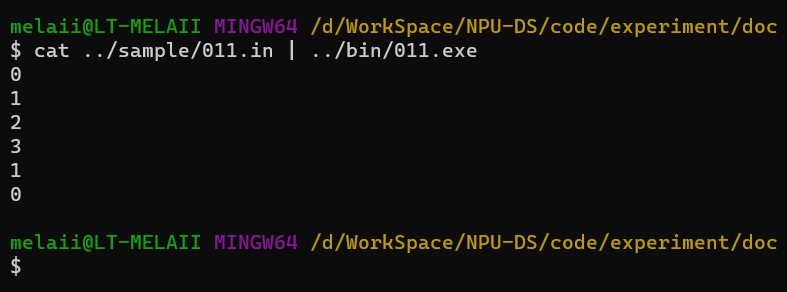
\includegraphics[width=125mm,height=48mm]{./assets/DS11-3}
		\caption{结果输出}
	\end{minipage}
\end{figure}

\subsection*{五、实验总结}
Floyd着实是一个暴力而美丽的算法,它是动态规划与贪心算法的结合,仅仅若干行的代码也使得其成为一个经典。简单描述,Floyd可用一个递推式概括:$d[i][j]=\mathop{min}\limits_{1\leq{k}\leq{n}}\{d[i][k]+d[k][j]\}$。虽然看上去很合理并可容易理解,但是仔细想想,在动态规划的过程中并不一定满足子问题已经最优,那么递推式还能够成立吗?查阅资料后我的答案是:成立。事实上,可以证明结论:假设i和j之间的最短路径上的结点集里(不包含i、j),编号最大的一个是v。那么在外循环k=v时,d[i][j]肯定得到了最小值。故而,这也是为什么对于中继节点的遍历必须位于外层而在内层会导致异常的原因。总结来讲,虽然该算法短得离谱,但是细细思索,依旧能够得到一些难关注到但是却极其关键的要素。

~\\
\zihao{-4}
\textbf{教师评语:}
~\\
\textbf{实验成绩:}

\begin{flushright}
\mbox{指导教师签名:\qquad\qquad} \\
\mbox{批阅日期:\qquad\qquad}
\end{flushright}

\end{document}